\begin{framecard}
	{\color{colorbg}
	\bfseries

	\hugetext{Open games with agency}}
\end{framecard}

\begin{frame}{What is a game?}
	\begin{quotation}
		\centering
		Game theory is the mathematical study of {\color<2->{colorarena}interaction}\\ among independent, self-interested {\color<2->{coloragents}agents}.\\
		{\color{colornote}-- Essentials of Game Theory \cite{leyton2008essentials}}
	\end{quotation}

	\vfill
	\begin{center}
		\alt<2->{
			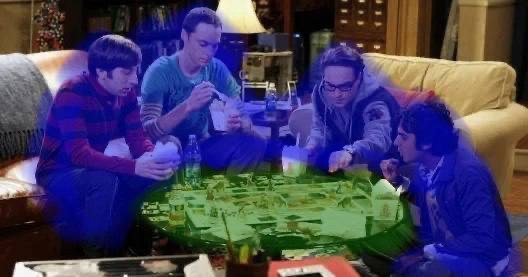
\includegraphics[width=.5\textwidth]{figures/board_games2.jpg}
		}{
			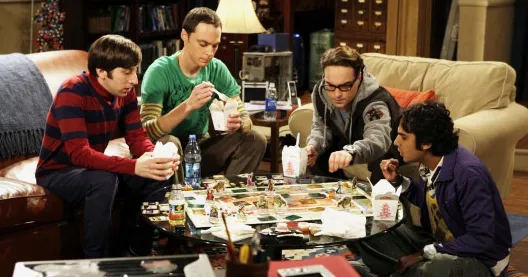
\includegraphics[width=.5\textwidth]{figures/board-games.png}
		}
	\end{center}

	\vfill
	\onslide<2->{
		A game factors in two parts:
		\begin{enumerate}
			\item An \textcolor{colorarena}{\textbf{arena}}, which models the \textbf{dynamics} of the game.
			\item \textcolor{coloragents}{\textbf{Players}}, which intervene in the arena by making \textbf{decisions} at different points.
		\end{enumerate}
	}

	\vfill
	\onslide<3->{
		A \textcolor{coloragents}{strategy} $\colag{\omega \in \Omega_p}$ for a player $\colag{}{1 \leq p \leq N}$ is a policy $p$ uses to make their decisions (e.g. a choice of move for each of $p$'s rounds).

		\vfill
		A \textcolor{coloragents}{strategy profile} is a strategy for each player $\colag{\Omega = \Omega_1 \times \cdots \times \Omega_p}$.
	}
\end{frame}

% rant about players here
\begin{frame}{What is a Nash equilibrium?}
	\begin{center}
		A strategy profile is a \textbf{Nash equilibrium}\\
		if no player has incentive to \emph{unilaterally} change strategy.
	\end{center}

	\vfill
	\begin{center}
		
\includegraphics[width=.7\textwidth]{figures/nash.png}
	\end{center}

	\vfill
	\textcolor{colornote}{Traditionally `the goal' of game theory is determining Nash equilibria of games, though this is not necessarily the case anymore (see: \cite{fudenberg1998theory}).}
\end{frame}

\begin{frame}{What is an arena?}
	An \textcolor{colorarena}{arena} is an open system with three boundaries:

	\begin{center}
		\includegraphics[clip, page=2, trim=0cm 3cm 3cm 2cm, width=.8\textwidth]{figures/drawings.pdf}
	\end{center}

	This is a parametrised lens $\textcolor{colorarena}{\A : (X,S) \nlongto{\textcolor{coloragents}{(\Omega, \Comega)}} (Y,R)}$ specified by two maps
	\begin{eqalign*}
		\textcolor{colorarena}{\play} &: \textcolor{coloragents}{\Omega} \textcolor{colorarena}{\times X \to Y},\\
		\textcolor{colorarena}{\coplay} &: \textcolor{coloragents}{\Omega} \textcolor{colorarena}{\times X \times R \to \textcolor{coloragents}{\Comega} \times S}
	\end{eqalign*}
\end{frame}

\begin{frame}{What is an arena?}
	It can be closed by specifying an \textbf{initial state} and a \textbf{utility function}:

	\begin{center}
		\fbox{\includegraphics[clip, page=4, trim=4.5cm 2cm 3cm 6cm, width=.9\textwidth]{figures/drawings.pdf}}
	\end{center}
\end{frame}

\begin{frame}{What is an arena?}
	At the end of the day, the \textcolor{colorarena}{arena} amounts to an evaluation of strategies with rewards:

	\vspace{5ex}
	\begin{center}
		\fbox{\includegraphics[clip, page=5, trim=3cm 7cm .5cm 5cm, width=.9\textwidth]{figures/drawings.pdf}}
	\end{center}
\end{frame}

\begin{frame}{What is a selection function?}
	\textcolor{coloragents}{Agents} express their preferences by means of a \textcolor{coloragents}{\textbf{selection function}}:

	{\fontsize{1.5em}{1.5em}\selectfont
	\begin{equation*}
		\colag{\varepsilon} : (\colar{\colag{\Omega} \to \colag{\Comega}}) \longto \copow{\colag \Omega}
	\end{equation*}
	}

	Typically, $\colag\Omega$ is 'finite', $\colag{\Comega = \R}$ and $\colag\varepsilon$ is $\argmax$:
	\begin{equation*}
		\colag{\argmax(\colar{u : \colag\Omega \to \colag\R})} = \{\colag{\omega \in \Omega} \suchthat \text{$\colag\omega$ maximises $\colar u$}\} \subseteq \colag\Omega.
	\end{equation*}

	\vfill
	\onslide<2->{
		The assignment $\colag{\S(\Omega,\Comega)} := (\colar{\colag{\Omega} \to \colag{\Comega}}) \longto \copow{\colag \Omega}$ is functorial on $\Lens$.

		\vfill
		Crucially, it admits a lax monoidal structure (\textbf{Nash product}):
		\begin{eqalign*}
			&\colag{- \boxtimes -} : \colag{\S(\Omega_1,\Comega_1)} \times \colag{\S(\Comega_1, \Comega_2)} \longto \colag{\S(\Omega_1 \times \Omega_2, \Comega_1 \times \Comega_2)}\\[1ex]
			&\colag{(\varepsilon \boxtimes \eta)}(\colar{u}) = \{ \colag{(\omega_1,\omega_2)} \suchthat \colag{\omega_1} \in \colag{\varepsilon}(\colar{u_1(-,\colag{\omega_2})})\ \text{and}\ \colag{\omega_2} \in \colag{\eta}(\colar{u_2(\colag{\omega_1}, -)})\}\\
			&\phantom{\colag{(\varepsilon \boxtimes \eta)}(\colar{u})} = \text{strategies s.t. `no agent wants to unilaterally deviate'}
		\end{eqalign*}
		where $\colar{u = (u_1,u_2) : \colag{\Omega_1} \times \colag{\Omega_2} \to \colag{\Comega_1} \times \colag{\Comega_2}}$.
	}
\end{frame}

% \begin{frame}{Interlude: selection functions}
% 	Let $\S(X,S) := (X \to S) \to \pow{X}$. This is a functor on lenses:
% 	\begin{eqalign*}
% 		\S(\alpha) : \S(X,S) &\longto \S(Y,R)\\
% 		\varepsilon &\longmapsto \lambda k \,.\, \{x \cmp \alpha \suchthat x \in \varepsilon(\alpha \cmp k)\}
% 	\end{eqalign*}
% 	where $\alpha : (X, S) \to (Y,R)$ and we implicitly used $\Lens((1,1),(Y,R)) \iso Y \to R$ and $\Lens((X,S),(1,1)) \iso X$:

% 	(drawing)

% 	This functor is lax monoidal (\textbf{Nash product}):
% 	\begin{eqalign*}
% 		- \boxtimes - : \S(X,S) \times \S(Y,R) &\longto \S(X \times Y, S \times R)\\
% 		(\varepsilon, \eta) &\longmapsto \lambda k \,.\, \{ (x,y) \suchthat x \in \varepsilon(k_1(x,y))\ \text{and}\ y \in \eta(k_2(x,y))\}
% 	\end{eqalign*}
% 	(drawing)

% 	\textcolor{colornote}{This yields a moncat $\Lens_\S = \underset{mon}\int \S$.}
% \end{frame}

\begin{frame}{The definition}
	\begin{definition}
		An \textbf{open game with agency} is a pair
		\begin{equation*}
			\G \quad = \quad (\ \colar{\A : (X,S) \nlongto{\colag{(\Omega, \Comega)}} (Y,R)}, \quad \colag{\varepsilon  : \S(\Omega, \Comega)}\ )
		\end{equation*}
		whose equilibria are given by
		\begin{equation*}
			\eq_\G(x, k) = \colag{\varepsilon(}\colar{x \cmp \A \cmp k}\colag{)}.
		\end{equation*}%
		\textcolor{colornote}{In this way we recover the equilibrium predicate of open games.}
	\end{definition}

	\vfill
	\onslide<2->{
		\begin{definition}
			$\G$ \textbf{has set of players $\colag P$} when
			\begin{equation*}
				\colag{
					\Omega = \prod_{p \in P} \Omega_p, \quad \Comega = \prod_{p \in P} \Comega_p, \quad \varepsilon = \Boxtimes_{p \in P} \varepsilon_p
				}
			\end{equation*}
			in which case
			\begin{equation*}
				\eq_\G(x, k) = \colag{(\varepsilon_1 \boxtimes \cdots \boxtimes \varepsilon_n)(}\colar{x \cmp \A \cmp k}\colag{)}.
			\end{equation*}
		\end{definition}
	}
	%where $(-)^\top : \Lens_{(\Omega, \Comega)}((1,1),(1,1))\ \iso\ \Omega \to \Comega$.
\end{frame}

% Let's focus on arenas, aka parametrised lenses, for a while...
\begin{frame}{Composing games}
	%\textcolor{colorarena}{Arenas} are the compositional heart of open games with agency:

	\begin{itemize}
		\item \textbf{Sequential composition}
		\begin{center}
			\includegraphics[clip, page=7, trim=0cm 21cm 0cm 2cm, width=.9\textwidth]{figures/drawings.pdf}
		\end{center}
		\item \textbf{Parallel composition}
		\begin{center}
			\includegraphics[clip, page=7, trim=0cm 5cm 0cm 13cm, width=.9\textwidth]{figures/drawings.pdf}
		\end{center}
	\end{itemize}

	\textbf{Notice}: these operators \underline{can} be extended to games:
	\begin{equation*}
		(\colar{\A_1}, \colag\varepsilon) \cmp (\colar{\A_2}, \colag\eta) := (\colar{\A_1 \cmp \A_2}, \colag{\varepsilon \boxtimes \eta}), \quad (\colar{\A_1}, \colag\varepsilon) \otimes (\colar{\A_2}, \colag\eta) := (\colar{\A_1 \otimes \A_2}, \colag{\varepsilon \boxtimes \eta})
	\end{equation*}
\end{frame}

\begin{frame}{Composing arenas}

	\begin{itemize}
		\item \textbf{External choice}
		\begin{center}
			\includegraphics[clip, page=8, trim=0cm 17cm 0cm 4cm, width=.9\textwidth]{figures/drawings.pdf}
		\end{center}
		The `environment' chooses which game to play, agents are prepared to play both.
		\item \textbf{Internal choice}
		\begin{center}
			\includegraphics[clip, page=8, trim=0cm 7cm 0cm 14cm, width=.9\textwidth]{figures/drawings.pdf}
		\end{center}
		The `environment' can play either game, agents choose which one.
	\end{itemize}

	\textbf{Notice}: these operators \underline{can't} be extended to selection functions in a canonical way! \textcolor{colornote}{(Actually $\oplus$ \underline{can} if we refine our typing judgments)}
\end{frame}

\begin{frame}{Reparametrisation}
	Most importantly arenas form a (locally fibred) bicategory: one can \textbf{reparametrise} along a lens $\colag{\alpha : (\Omega', \Comega') \to (\Omega, \Comega)}$.

	\begin{center}
		\includegraphics[clip, page=9, trim=0cm 7cm 0cm 14cm, width=.9\textwidth]{figures/drawings.pdf}
	\end{center}

	\vfill
	This is crucial for introducing agency!

	%\vfill
	%\textcolor{colornote}{If we work in $\Para_{\times_\S}(\Lens_\S)$, we see that `$(1,1,\top)$ coclassifies equilibria', i.e. $(1,1,\top) \twoto \G \iso \eq_\G$.}
\end{frame}

\begin{frame}{Regrouping}
	If $\A$ has set of players $P$ and $r : P \to Q$ is a function, we can turn $\A$ into an arena with players $Q$ by reparametrising along
	\begin{equation*}
		\colag{\regroup_r : ({\textstyle\prod}_{q \in Q} (r^* \Omega)_q, {\textstyle\prod}_{q \in Q} (r^* \Comega)_q) \longto ({\textstyle\prod}_{p \in P} \Omega_p, {\textstyle\prod}_{p \in P} \Comega_p)}
	\end{equation*}
	which only permutes \& reindex the factors according to $r$.
	\begin{example}
		If $\colar{\A_1}$ and $\colar{\A_2}$ have the same players $\colag P$, $\colar{\A_1 \cmp \A_2}$ has players $\colag{P+P}$. So we regroup along $\colag{P+P \to P}$ to get again an arena with players $P$.
	\end{example}
	(drawing)
\end{frame}

\begin{frame}{Tying}
	The second most important application for reparametrisations is tying strategies at different point of the game. This is done by reparametrising along $\colag{(\Delta, \mathsf{combine})}$ (where $\colag{\mathsf{combine} = +, \pi_2, \max, \ldots}$).

	\vfill
	\textbf{Notice}: $\colag{(\Delta, \mathsf{combine})^*}\colar{(\A_1 \cmp \A_2)}$ lies outside the image of $-\cmp-$, hence introduces 'non-compositional' effects. Indeed: \textbf{\textcolor{coloragents}{agency} is non-local.}
	%\textcolor{colornote}{We'll use this soon to treat imperfect information. Also useful for Markov games.}
\end{frame}
